
\begin{figure}
	\centering
	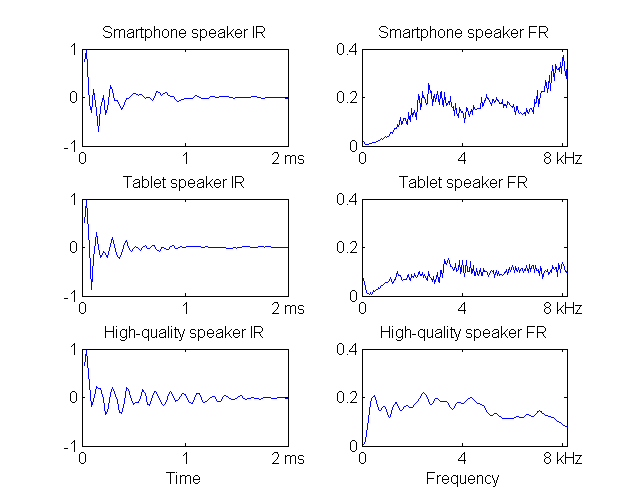
\includegraphics[width=1\linewidth]{Figs/IRs.png}
	\caption{Impulse (left) and frequency (right) responses for three different loudspeakers.}
	\label{fig::IRs}
\end{figure}

Replay attacks are emulated according to the approach described in Section~\ref{ssec:replay} 
%{\bfseries Needed here is an explanation of why you ignored $mic(t)$ and $a(t)$.}  
%Emulations include
using a random mix of three different loudspeaker impulse responses $\mathrm{spk}(t)$ and three different replay environments $b(t)$.  
%The worst-case scenarios is again considered, i.e., the case where the spoofer possesses a high-quality recording of the target speaker.  Accordingly, $mic(t)$ and $a(t)$ in Equation~\ref{eq::playback} are not considered.  While $a(t)$ can impact on results, as in the case of far-field recordings, loudspeaker effects are known to dominate microphone effects.  Omission of $mic(t)$ is therefore likely to be inconsequential.
Speaker impulse responses $\mathrm{spk}(t)$ are obtained from~\cite{Brown2014} and correspond to a low-quality smartphone speaker, a medium-quality tablet speaker and a high-quality stand-alone speaker.  The impulse response and frequency responses of each are illustrated in Fig.~\ref{fig::IRs}.  There are significant differences in the frequency responses which show in particular the high-pass functions of the smaller (and perhaps lower quality) devices.  The third impulse response is comparatively flat, though with greater high-frequency attenuation.  The first two impulse responses are, however, comparatively short, whereas the third extends to 2ms.  The first two replay environment impulse responses $b(t)$ are obtained from~\cite{Jeub2009} and correspond to an enclosed medium-sized office and an open corridor. The impulse and frequency responses of each are illustrated in Fig.~\ref{fig::Room_IRs}.  The impulse responses are significantly longer in duration than those of the loudspeakers.  The frequency responses also exhibit greater variation.  The third impulse response simulates an anechoic chamber with a flat frequency response.  This particular setup is necessary in order to assess the importance of a real the acoustic environment and its importance as a means of detecting replay spoofing attacks.

This approach to generate spoofing attacks through emulation might seem undesirable at first.  However, given representative impulse responses and a time-invariant linear system, then genuine recordings will produce replay attacks that are entirely equivalent to those obtained through emulation.  The impact of emulation on the findings of this work is thus negligible.  Furthermore, the emulation approach permits a study with many more replay and acoustic environments than would otherwise be practicable with a genuine setup.  The emulation approach thus has significant merit for this and future work.


\begin{figure}
	\centering
	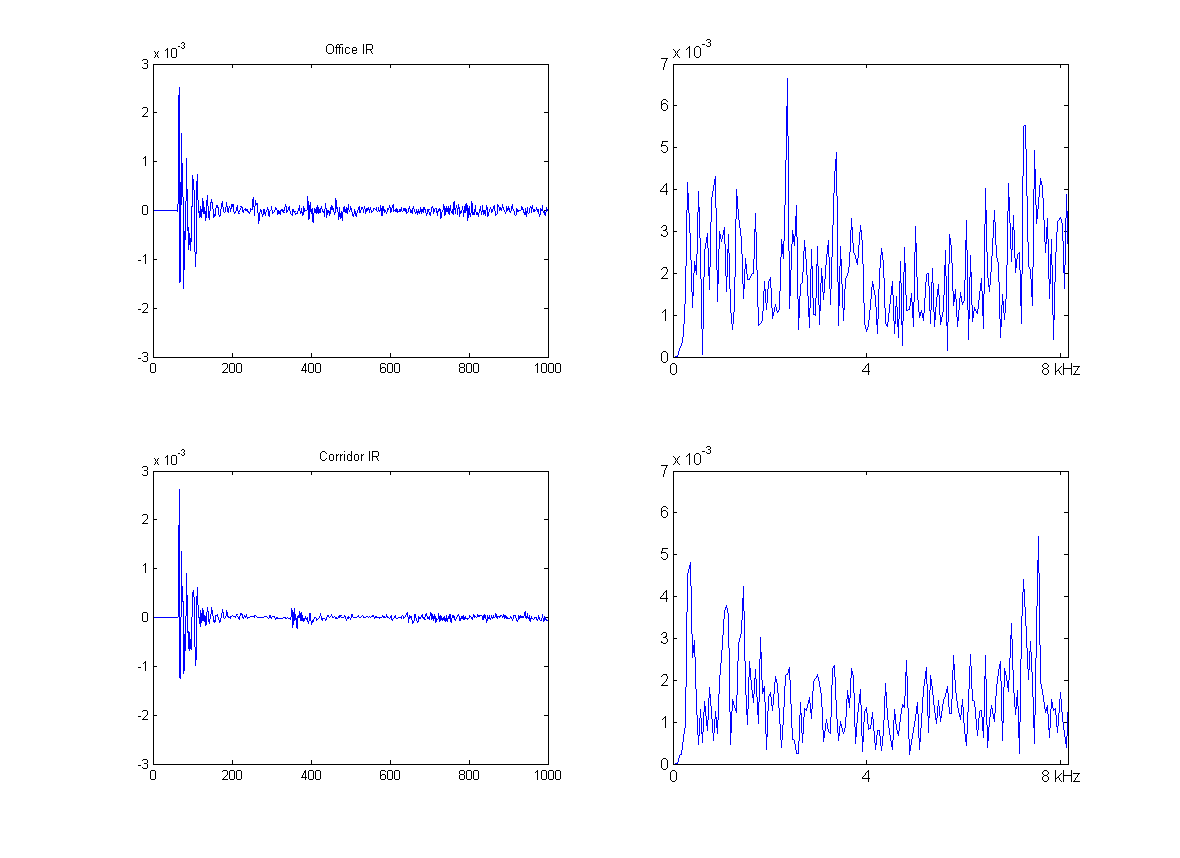
\includegraphics[width=1\linewidth]{Figs/Room_IRs.png}
	\caption{Impulse (left) and frequency (right) responses for two different acoustic environments.}
	\label{fig::Room_IRs}
\end{figure}


%{\bfseries One potential problem here: in the use case relevant to this work, voice conversion speech synthesis and replay attacks will all involve replay, and thus a particular $b(t)$, yet your experiments only consider $b(t)$ for replay.  The comparison is therefore not fair.  I suggest to remove $b(t)$ in your replay work.  In any case there is no difference between the two impulse responses.}

%{\bfseries [AJ] I think this is not always the case. We can easily imagine a VC or SS application running on a smartphone and emitting converted/synthetic voice directly to the telephone channel. Or a hardware gadget which is plugged to a smartphone instead of a headset -- there's no replay here either. If replay is involved, efficiency of SS or VC attack is even lower. Without considering $b(t)$ for them we in fact work in favour of them. In the replay attack, in the simplest usage case you don't use any dedicated applications, this is why we have to consider $b(t)$. Besides, the difference between them is remarkable, see the results in Table~\ref{tab::results_CM_rooms} and Table~\ref{tab::results_EER}.}
